\chapter{Experiments} \label{chap:exp}

In order to evaluate our proposed algorithms, the heuristic balancing method (\emph{GM}), the distance based node clustering scheme (\emph{DIST}), as well as the combination of those (\emph{HDM}), we compare them with the geometric monitoring method~\cite{Sharfman2006GM}, hereby refered to as \emph{GM}, and the hierarchical clustering method of~\cite{Keren2014GMHetStreams}, hereby refered to as \emph{DISTR}. Datasets originate from both synthetic and real-world settings in order to explore the performance, scalability and applicability of our methods in terms of reduction in communication.

Firstly, Section~\ref{sec:datasets} contains a detailed description of the datasets and the monitoring functions used for evaluation purposes. Following that, Section~\ref{sec:exp} presents the experimental results along with the necessary commentation.

\section{Data, Setup and Monitoring Functions} \label{sec:datasets}

\subsection{Synthetic Datasets}

Synthetic datasets have been incorporated into the evaluation process of the proposed algorithms in order to provide a controlable environment under which the behaviour of our methods can be analyzed. Data streams are created by firstly sampling data stream velocity distribution means by a user specified normal distribution and fixing the standard deviation of each stream. Afterwards, an initial velocity is sampled from each stream's assigned distribution and a $\lambda$ value is chosen, which controls the rate of change of the streams' velocity. Stream update $v_i(t_k)$ of node $n_i$ at time $t_k$ is generated by sampling a new velocity $u_{k+1}$ from the velocity distribution assigned to node $n_i$ and updating the streams' value by: $v_i(t_{k+1})=v_i(k) + (1-\lambda)u_{k} + \lambda u_{k+1}$. Noisy versions of the generated streams are the product of additive Gaussian noise.

Linear streams (\emph{LIN}) are generated by setting the parent distribution to $\mathcal{N}(10,20)$, the standard deviation of each stream's velocity distribution to $\sigma=10$ and the lambda value to $\lambda=0$. An example of the resulting one dimensional streams corresponding to 20 nodes, along with the resulting global statistics stream, is illustrated in Figure~\ref{fig:linearStreams}.

Interweaving streams(\emph{INT}) are produced from the same parent distribution $\mathcal{N}(10,20)$ by selecting $\sigma=50$ for the standard deviation of each stream's velocity distribution and $\lambda=0.1$ as the velocity update parameter. An instance of one dimensional interweaving streams corresponding to 20 nodes, along with the resulting global statistics stream, is shown in Figure~\ref{fig:intStreams}.

Noisy streams (\emph{NOISE}) are the result of the previously used parent distribution with $\sigma=100$ as the standard deviation of each stream's velocity, $\lambda=0.15$ the velocity update parameter, and  $\mathcal{N}(0,30)$ the distribution of the additive Gaussian noise. Such one dimensional streams corresponding to 20 monitoring nodes, along with the resulting global statistics stream, is depicted in Figure~\ref{fig:noiseStreams}.

%%%%%%%%%%%%%%%%%%%%%%%%%%%%%%%%%LIN synthetic datasets figure %%%%%%%%%%%%%%%%%%%%%%%%%%%%
\begin{figure*}[t!]
\centering
\begin{subfigure}[t]{0.49\textwidth}
\centering
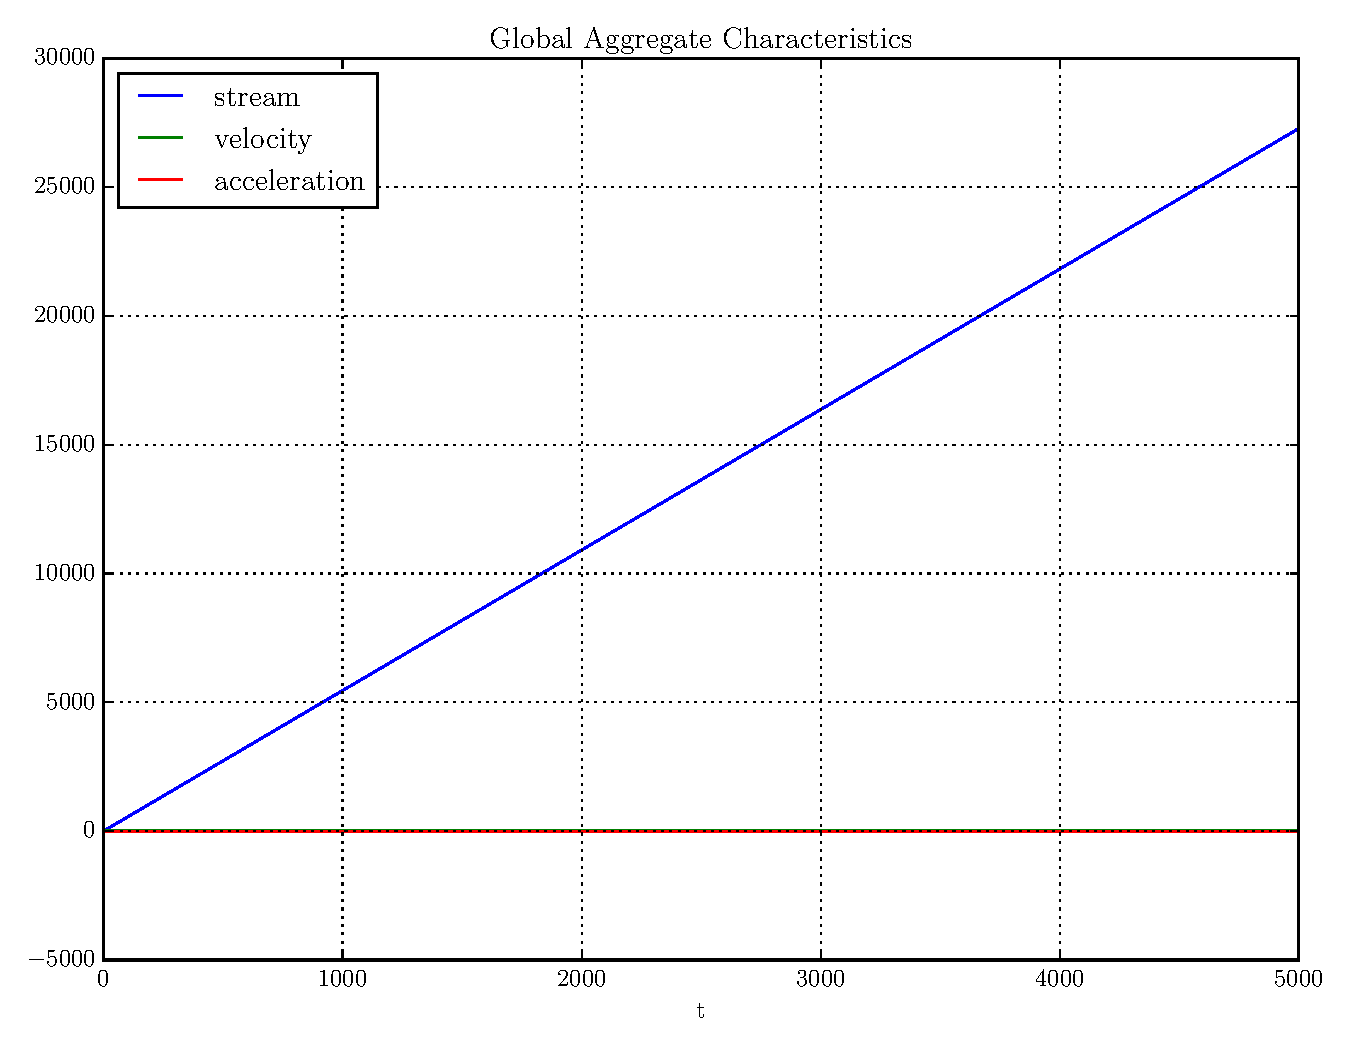
\includegraphics[scale=0.38, trim=2cm 0 0 0]{img/linear1D20N_global.pdf}
\caption{LIN global statistics stream of 20 streams}
\end{subfigure}
\begin{subfigure}[t]{0.49\textwidth}
\centering
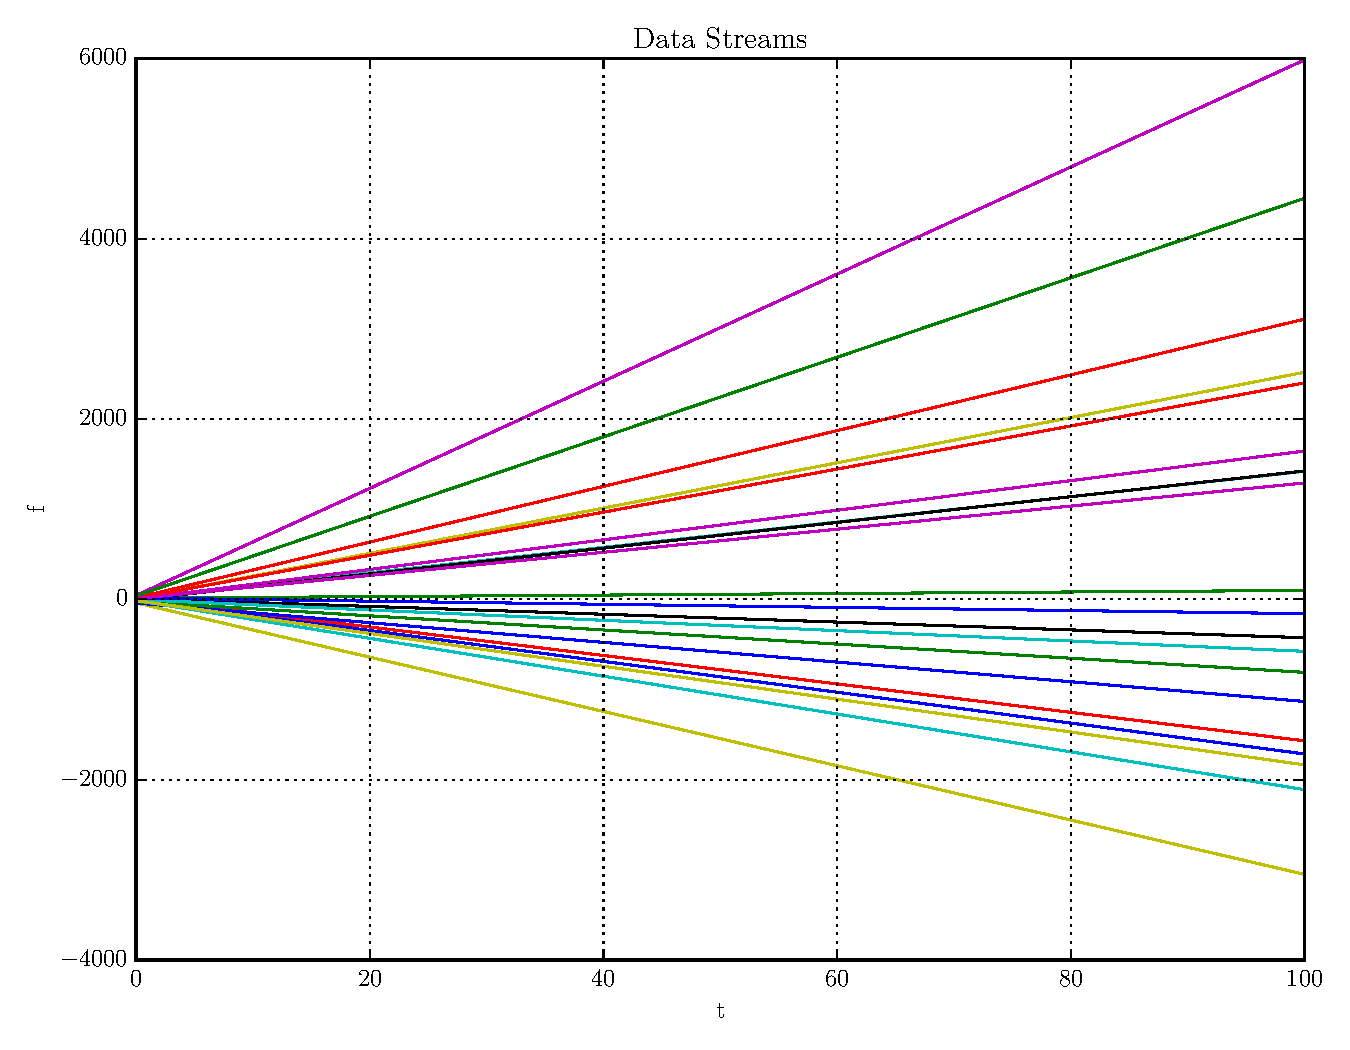
\includegraphics[scale=0.38]{img/linear1D20N_streams.pdf}
\caption{LIN local statistics streams for 20 nodes} 
\end{subfigure}
\vspace{0.5cm}
\caption{Linear data stream examples (LIN)}\label{fig:linearStreams}
\end{figure*}
%%%%%%%%%%%%%%%%%%%%%%%%%%%%%%%%%%%%%%%%%%%%%%%%%%%%%%%%%%%%%%%%%%%%%%%%%%%%%%%%%%%%%%%%%%%

%%%%%%%%%%%%%%%%%%%%%%%%%%%%%%%%%INT synthetic datasets figure %%%%%%%%%%%%%%%%%%%%%%%%%%%%
\begin{figure*}[t!]
\centering
\begin{subfigure}[t]{0.49\textwidth}
\centering
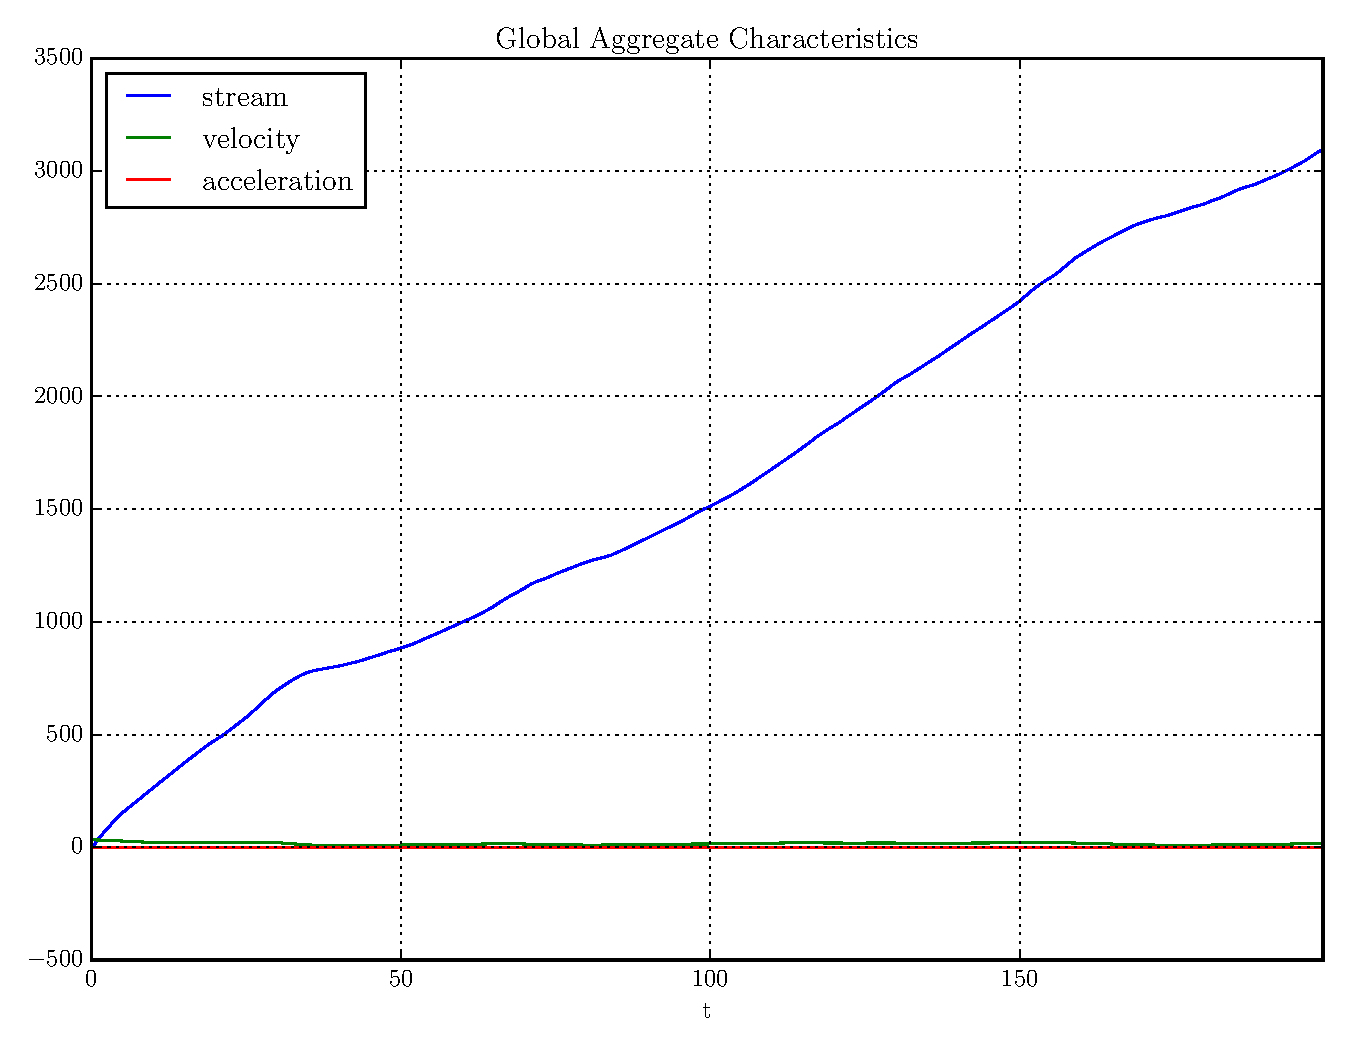
\includegraphics[scale=0.38, trim=2cm 0 0 0]{img/interweaving1D20N_global.pdf}
\caption{INT global statistics stream of 20 streams}
\end{subfigure}
\begin{subfigure}[t]{0.49\textwidth}
\centering
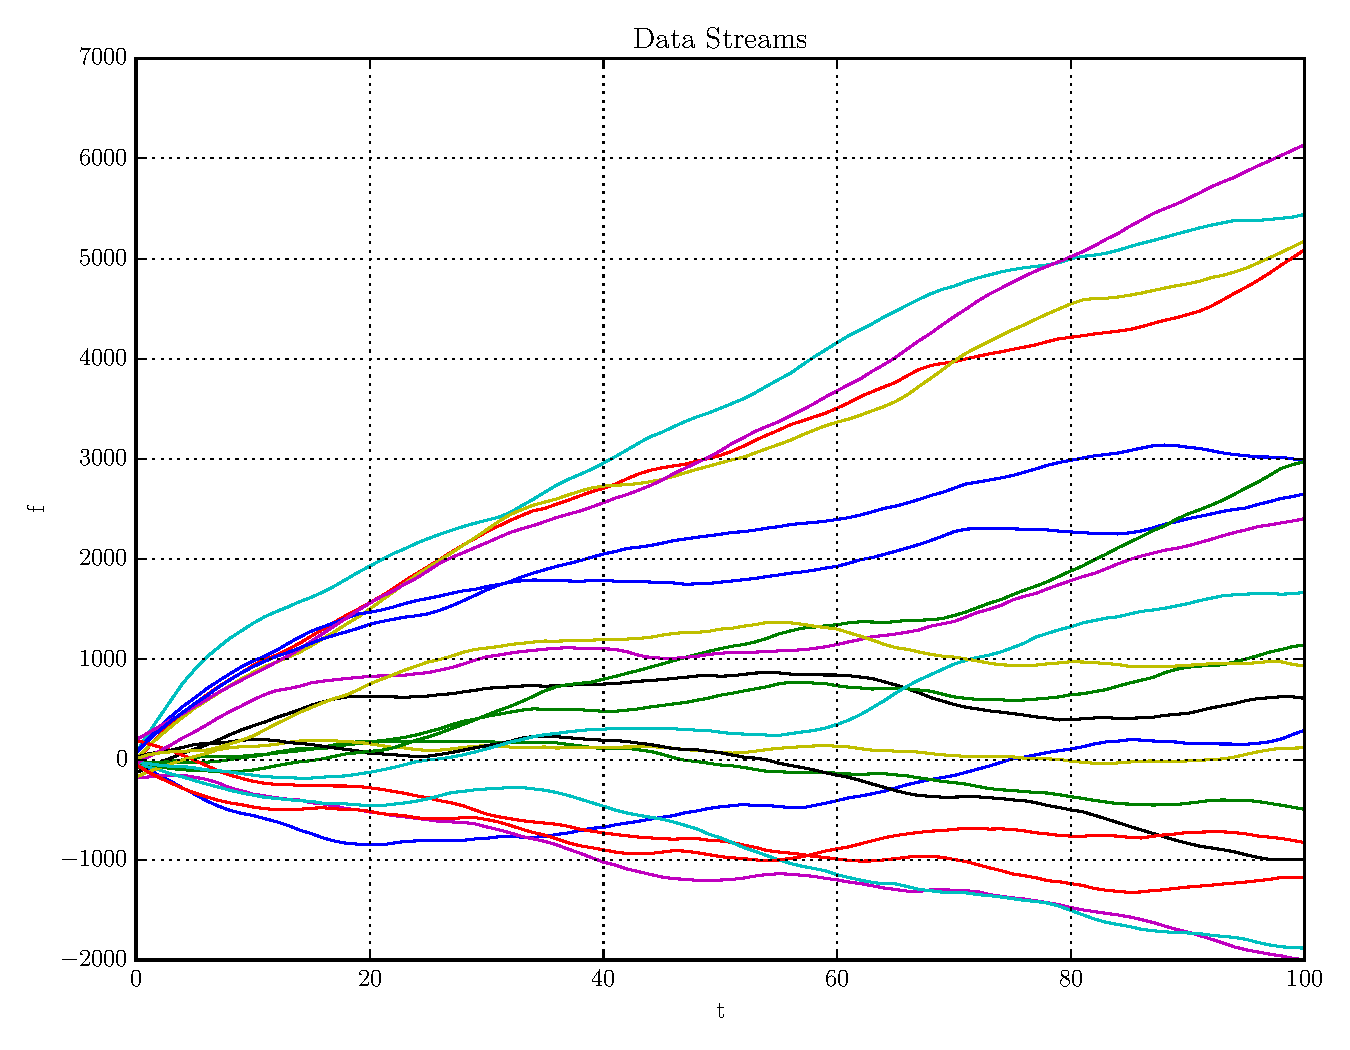
\includegraphics[scale=0.38]{img/interweaving1D20N_streams.pdf}
\caption{INT local statistics streams for 20 nodes} 
\end{subfigure}
\vspace{0.5cm}
\caption{Interweaving data stream examples (INT)}\label{fig:intStreams}
\end{figure*}
%%%%%%%%%%%%%%%%%%%%%%%%%%%%%%%%%%%%%%%%%%%%%%%%%%%%%%%%%%%%%%%%%%%%%%%%%%%%%%%%%%%%%%%%%%%

%%%%%%%%%%%%%%%%%%%%%%%%%%%%%%%%NOISE synthetic datasets figure %%%%%%%%%%%%%%%%%%%%%%%%%%%%
\begin{figure*}[t!]
\centering
\begin{subfigure}[t]{0.49\textwidth}
\centering
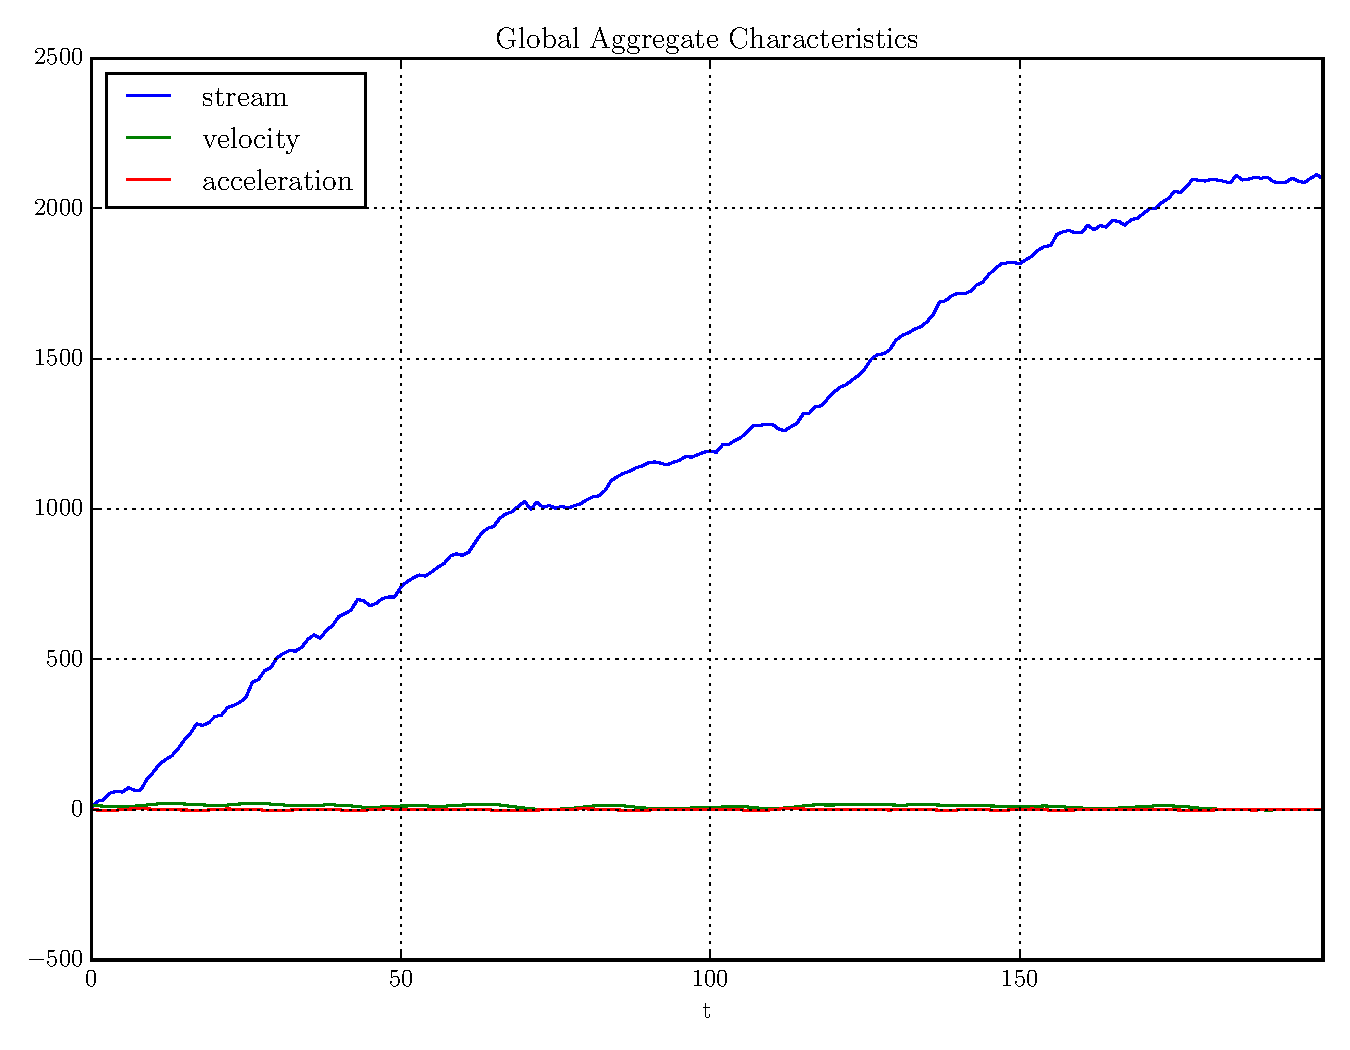
\includegraphics[scale=0.38, trim=2cm 0 0 0]{img/noisyinterweaving1D20N_global.pdf}
\caption{NOISE global statistics stream of 20 streams}
\end{subfigure}
\begin{subfigure}[t]{0.49\textwidth}
\centering
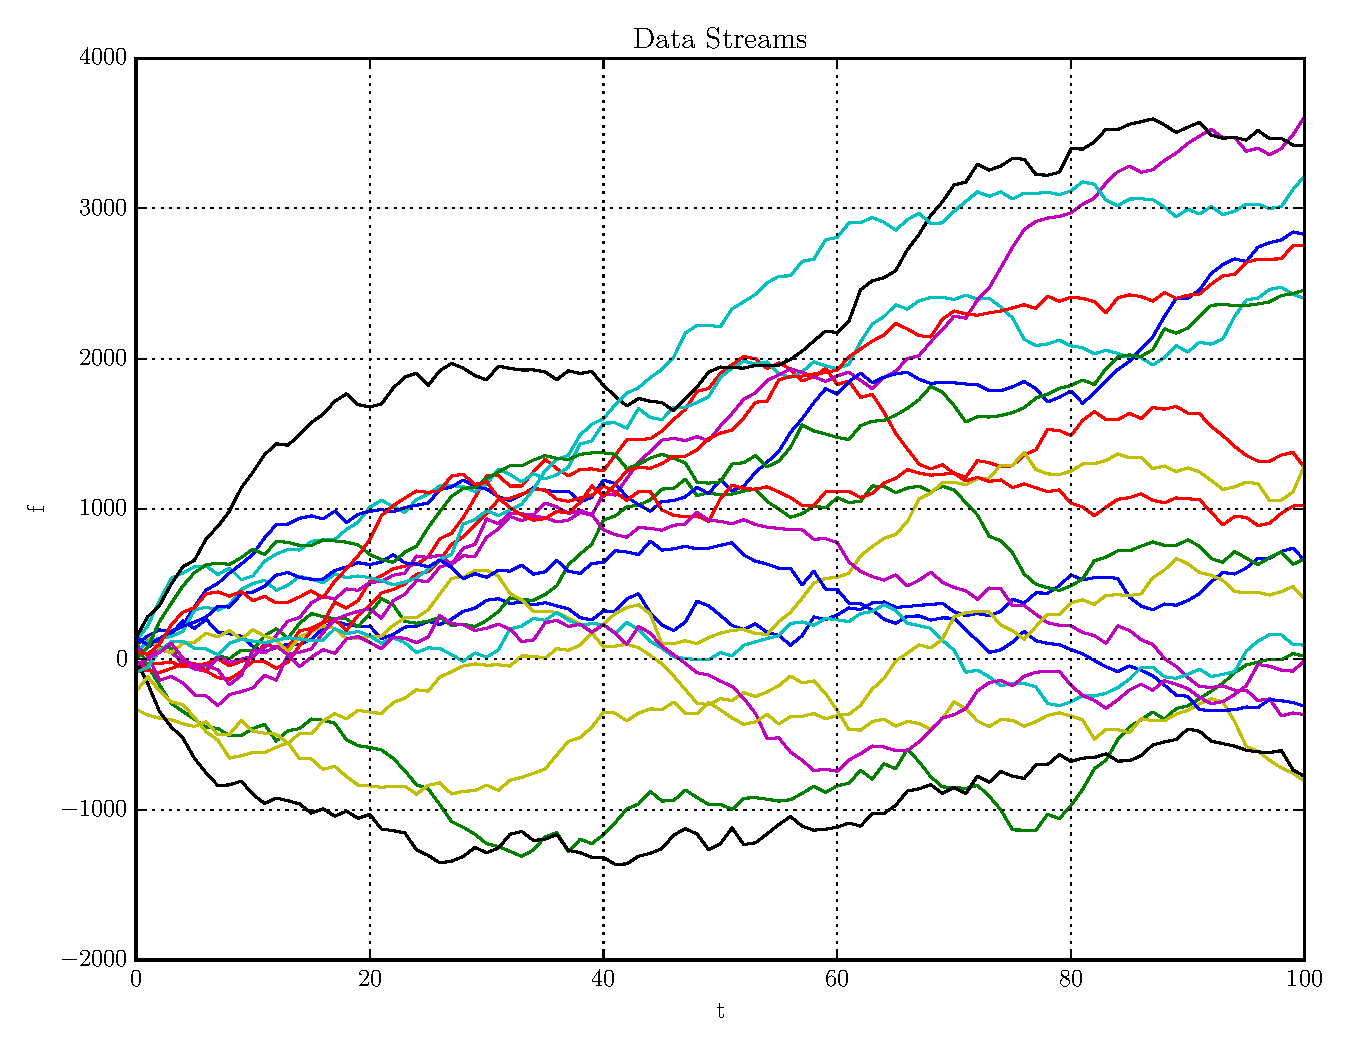
\includegraphics[scale=0.38]{img/noisyinterweaving1D20N_streams.pdf}
\caption{NOISE local statistics streams for 20 nodes} 
\end{subfigure}
\vspace{0.5cm}
\caption{Interweaving data stream examples (NOISE)}\label{fig:noiseStreams}
\end{figure*}
%%%%%%%%%%%%%%%%%%%%%%%%%%%%%%%%%%%%%%%%%%%%%%%%%%%%%%%%%%%%%%%%%%%%%%%%%%%%%%%%%%%%%%%%%%%


%TODO: include actual dataset?
\subsection{Air Quality Database}

what is air quality database

how were the streams formed and why

chosen functions

*images

\section{Experimental Results} \label{sec:exp}

\subsection{Node Matching Algorithms}

compare distance based node matching to distribution based node matching and the random selection algorithm with the classic balancing method

*images

\subsection{Balancing methods}

compare classic balancing with heuristic balancing with random selection algorithm

*images

\subsection{Monitoring Synthetic Data}

compare classic random with heuristic distance based matching over a range of nodes, a range of window sizes and a range of orders for SG

*images

%TODO:actual data?
\subsection{Monitoring Air Quality Data}

compare classic random with heristic distance based matching for the actual data, over a range of nodes and sg parameters to check how it affects performance

actual data streams that have great variance and irregularities lead to poor proposed algorithm performance

*images
